\documentclass[12pt,a4paper]{article}
\usepackage[utf8]{inputenc}
\usepackage[T2A]{fontenc}
\usepackage[english,russian]{babel}
\usepackage[a4paper, mag=1000, left=1.5cm, right=2cm, top=2cm, bottom=2cm, headsep=0.7cm, footskip=1cm]{geometry}
\usepackage{amsmath}
\usepackage{pgfplots, colortbl}
\usepackage{makecell}
\usepackage{multicol}
\usepackage{pgfplotstable}
\pgfplotsset{compat=1.16}
\usepackage{minted}
\usepackage{listings}
\usepackage{lstfiracode}
\usepackage{caption}
\usepackage{mathrsfs}
\usepackage{placeins}
\usepackage{graphicx}

\usemintedstyle{colorful}
\newenvironment{code}{\captionsetup{type=listing}}{}


\newcommand{\itertable}[2]{
	\FloatBarrier
	\begin{table}[h]
		\centering
		\caption*{Количество итераций}
		\pgfplotstabletypeset[
			every even row/.style=
				{before row={\rowcolor[gray]{0.95}}},
			string type,
			columns/point/.style={column name=Начальная точка, column type={|c|}},
			columns/f1/.style={column name=$f_1$, column type={c|}},
			columns/f2/.style={column name=$f_2$, column type={c|}},
			columns/f3/.style={column name=$f_3$, column type={c|}},
			columns/f4/.style={column name=$f_4$, column type={c|}},
			every head row/.style={before row=\hline, after row=\hline},
			every last row/.style={after row=\hline}
		]{#1}
	\end{table}
	\FloatBarrier
}

\newcommand{\dtable}[2]{
	\FloatBarrier
	\begin{table}[h]
		\centering
		\caption*{#2}
		\pgfplotstabletypeset[
			every even row/.style=
			{before row={\rowcolor[gray]{0.95}}},
			string type,
			columns/iter/.style={column name=$№$, column type={|c|}},
			columns/iter/.style={column name=$\alpha$, column type={c|}},
			every head row/.style={before row=\hline, after row=\hline},
			every last row/.style={after row=\hline}
		]{#1}
	\end{table}
	\FloatBarrier
}

\newcommand{\methodtable}[2]{
	\FloatBarrier
	\begin{table}[h]
		\centering
		\caption*{Количество итераций}
		\pgfplotstabletypeset[
			every even row/.style=
			{before row={\rowcolor[gray]{0.95}}},
			string type,
			columns/method/.style={column name=Метод, column type={|c|}},
			columns/f1/.style={column name=$f_1$, column type={c|}},
			columns/f2/.style={column name=$f_2$, column type={c|}},
			every head row/.style={before row=\hline, after row=\hline},
			every last row/.style={after row=\hline}
		]{#1}
	\end{table}
	\FloatBarrier
}


\newcommand{\fullgraph}[4]{
	\begin{center}
		\begin{tikzpicture}
			\begin{axis}[
					title = {График зависимости логарифма относительной погрешности от $k$},
					xlabel = $k$,
					ylabel = \(\log \delta x\),
					legend pos=outer north east,
					ylabel style={rotate=-90},
					ymode = log
				]
				\addplot table [x={k}, y={rel}, /pgf/number format/read comma as period] {data/task2/n#1.csv};
				\addplot table [x={k}, y={rel}, /pgf/number format/read comma as period] {data/task2/n#2.csv};
				\addplot table [x={k}, y={rel}, /pgf/number format/read comma as period] {data/task2/n#3.csv};
				\addplot table [x={k}, y={rel}, /pgf/number format/read comma as period] {data/task2/n#4.csv};
				\addlegendentry{$n = #1$}
				\addlegendentry{$n = #2$}
				\addlegendentry{$n = #3$}
				\addlegendentry{$n = #4$}
			\end{axis}
		\end{tikzpicture}
		\begin{tikzpicture}
			\begin{axis}[
					title = {График зависимости логарифма относительной погрешности от $cond$},
					xlabel = $\log cond$,
					ylabel = \(\log \delta x\),
					legend pos=outer north east,
					ylabel style={rotate=-90},
					xmode = log,
					ymode = log,
				]
				\addplot table [x={cond}, y={rel}, /pgf/number format/read comma as period] {data/task2/n#1.csv};
				\addplot table [x={cond}, y={rel}, /pgf/number format/read comma as period] {data/task2/n#2.csv};
				\addplot table [x={cond}, y={rel}, /pgf/number format/read comma as period] {data/task2/n#3.csv};
				\addplot table [x={cond}, y={rel}, /pgf/number format/read comma as period] {data/task2/n#4.csv};
				\addlegendentry{$n = #1$}
				\addlegendentry{$n = #2$}
				\addlegendentry{$n = #3$}
				\addlegendentry{$n = #4$}
			\end{axis}
		\end{tikzpicture}
	\end{center}
}

\newcommand{\graph}[1]{
	\begin{center}
		\begin{tikzpicture}
			\begin{axis}[
					title = {График зависимости логарифма относительной погрешности от размерности матрицы},
					xlabel = $n$,
					ylabel = \(\log \delta x\),
					ylabel style={rotate=-90},
					ymode = log
				]
				\addplot table [x={n}, y={rel}, /pgf/number format/read comma as period] {#1};
			\end{axis}
		\end{tikzpicture}
	\end{center}
}

\newcommand{\loggraph}[3]{
	\begin{center}
		\begin{tikzpicture}
			\begin{semilogxaxis}[
					title = {График зависимости количества итераций метода от размерности},
					xlabel = $\log n$,
					ylabel = \(\log iterations\),
					ylabel style={rotate=-90},
					ymode = log,
					legend pos=outer north east
				]
				\addplot table [x={n}, y={iter}, /pgf/number format/read comma as period] {#1};
				\addplot table [x={n}, y={iter}, /pgf/number format/read comma as period] {#2};
				\addplot table [x={n}, y={iter}, /pgf/number format/read comma as period] {#3};
				\addlegendentry{диагональное преобладание}
				\addlegendentry{обратный знак}
				\addlegendentry{матрицы Гильберта}
			\end{semilogxaxis}
		\end{tikzpicture}
	\end{center}
}

\newcommand{\densegraph}[2]{
	\begin{center}
		\begin{tikzpicture}
			\begin{axis}[
					title = {График зависимости логарифма относительной погрешности от размерности матрицы},
					xlabel = $n$,
					ylabel = \(\log \delta x\),
					legend pos=outer north east,
					ylabel style={rotate=-90}
				]
				\addplot table [x={n}, y={rel}, /pgf/number format/read comma as period] {#1};
				\addplot table [x={n}, y={rel}, /pgf/number format/read comma as period] {#2};
				\addlegendentry{метод Гаусса для плотных матриц}
				\addlegendentry{метод Гаусса для LU-разложения}
			\end{axis}
		\end{tikzpicture}
	\end{center}
}


\newcommand{\img}[1] {
	\begin{center}
		\includegraphics[width=.7\linewidth, height=.4\textheight]{#1}
	\end{center}
}
\newcommand{\mcode}[2]{
	\begin{code}
		\caption*{#1}
		\inputminted[breaklines=true, xleftmargin=1em, linenos, frame=single, framesep=10pt, fontsize=\footnotesize]{java}{path}
	\end{code}
	\newpage
}


\begin{document}

\begin{titlepage}
	\begin{center}
		\textsc{Национальный исследовательский университет ИТМО\\
			Прикладная математика и информатика}\\[5cm]

		\huge{Методы оптимизации\\[6mm]
			\large Отчет по лабораторной работе №2\\
			``Алгоритмы минимизации многомерных функций''\\[4cm]

		}
	\end{center}

	\begin{flushright}
		\begin{minipage}{0.25\textwidth}
			Выполнили:\\[2mm]
			Михайлов Максим\\
			Загребина Мария\\
			Кулагин Ярослав\\[2mm]
			Команда:

			\(\forall \bar R \in \mathscr{R}^n : \mathrm{\textbf{R}}(\bar R) \in \mathscr{R}\)

			(КаМаЗ)\\[2mm]
			Группа: M3237
		\end{minipage}
	\end{flushright}

	\vfill
	\begin{center}
		Санкт-Петербург, \today
	\end{center}
\end{titlepage}



\section{Цели}
\begin{enumerate}
	\item Реализовать алгоритмы минимизации функций:
	      \begin{itemize}
		      \item Метод градиентного спуска
		      \item Метод наискорейшего спуска
		      \item Метод сопряженных градиентов
	      \end{itemize}
	\item Исследовать скорость сходимости в зависимости от выбора алгоритма одномерной оптимизации в методе наискорейшего спуска.
	\item Проанализировать траектории методов на различных квадратичных функциях
	\item Исследовать зависимость числа итераций от следующих входных параметров:
	      \begin{itemize}
		      \item Число обусловленности
		      \item Размерность пространства
	      \end{itemize}
\end{enumerate}

\section{Вычислительная схема методов}

\subsection{Метод градиентного спуска}

Алгоритм метода:
\begin{enumerate}
	\item Выбрать \(\varepsilon > 0, \alpha > 0, x\in E_n\), вычислить \(f(x)\).
	\item Вычислить \(\nabla f(x)\). Проверить условие \(||\nabla f(x)|| < \varepsilon\). Если оно выполнено, то завершить процесс, иначе перейти к шагу 3.
	\item Найти \(y = x - \alpha \nabla f(x)\) и \(f(y)\). Если \(f(y) < f(x)\), принимаем \(\alpha = \frac{\alpha}{2}\) и выполняем этот шаг ещё раз. Иначе положить \(x = y, f(x) = f(y)\) и перейти к шагу 2.
\end{enumerate}

\subsection{Метод наискорейшего спуска}

Алгоритм метода:
\begin{enumerate}
	\item Выбрать \(\varepsilon > 0, x \in E_n\), вычислить \(f(x)\)
	\item Вычислить \(\nabla f(x)\). Проверить условие \(||\nabla f(x)|| < \varepsilon\). Если оно выполнено, то завершить процесс, иначе перейти к шагу 3.
	\item Решить задачу одномерной оптимизации
	      \[\Phi(\alpha) \to \min \quad \Phi(\alpha) = f(x - \alpha \nabla f(x)), \alpha > 0\]
	      Положить \(x = x - \alpha \nabla f(x)\), перейти к шагу 2.
\end{enumerate}

\subsection{Метод сопряженных градиентов}

Алгоритм метода:
\begin{enumerate}
	\item Выбрать \(\varepsilon > 0, x \in E_n\), вычислить \(\nabla f(x)\), задать \(p = -\nabla f(x)\)
	\item Вычислить \(\nabla f(x)\). Проверить условие \(||\nabla f(x)|| < \varepsilon\). Если оно выполнено, то завершить процесс, иначе перейти к шагу 3.
	\item Вычислить следующие значения:
	      \[t = Ap\]
	      \[\alpha = \frac{||\nabla f(x)||^2}{\langle t, p\rangle} \]
	      \[\tilde{x} = x + \alpha \cdot p\]
	      \[\nabla f(\tilde{x}) = \nabla f(x) + \alpha \cdot t\]
	      \[\beta = \frac{||\nabla f(\tilde{x})||^2}{||\nabla f(x)||^2}\]
	      \[p = - \nabla f(\tilde{x}) + p \cdot \beta\]

	      И принять \(\tilde{x}\) за \(x\), \(\nabla f(\tilde{x})\) за \(\nabla f(x)\)
\end{enumerate}

\section{Ход работы}

\subsection{Скорость сходимости в зависимости от выбора алгоритма одномерной оптимизации}

Следующие измерения проводились для функции \(f = x^2 + y^2 - xy + 4x + 3y - 1\) с начальной точкой \((2, 2)\), искомой точностью \(\varepsilon = 10^{ - 6}\).

Аналитическое решение задачи:
\begin{align*}
	 & \begin{cases}
		f'_x = 2x - y + 4 \\
		f'_y = 2y - x + 3
	\end{cases}  & \\
	 & \begin{cases}
		0 = 2x - y + 4 \\
		0 = 2y - x + 3
	\end{cases}   \\
	 & \begin{cases} x = - \frac{11}{3} \\ y = - \frac{10}{3} \end{cases}
\end{align*}


\begin{enumerate}
	\item Метод золотого сечения \\
	      \\
	      \funtable{dichotomy} \\
	\item Метод фибоначчи \\
	      \\
	      \funtable{fibonacci}
	\item Метод золотого сечения \\
	      \\
	      \funtable{golden_ratio}
	\item Метод Брента \\
	      \\
	      \funtable{brent}
\end{enumerate}

Таким образом, количество итераций метода наискорейшего спуска не зависит от выбора способа одномерного поиска, но это влияет на скорость работы. Метод парабол не работает для данной функции, т.к. при одномерной оптимизации используется функция с минимумом на границе отрезка допустимых решений. Такие функции не оптимизируются методом парабол, в силу невозможности найти начальное приближение \(\tilde{x}\) такое, что \(f(x_1) \leq f(\tilde{x})\), \(f(x_2) \geq f(\tilde{x})\), \(\tilde{x} \neq x_1\), \(\tilde{x} \neq x_2\), где \(x_1, x_2\) --- границы отрезка, на котором производится оптимизация.

\subsection{Траектории методов на различных функциях}
Во всех вычислениях для алгоритма наискорейшего спуска использовался метод Брента.\\
$\varepsilon = 10^{-6}$ \\
Начальная точка (-3, 3) \\

\begin{enumerate}
	\item \(f_1 = x^2 + y^2 - xy + 4x + 3y - 1\) \\
	      Точка минимума \(\left( - \frac{11}{3}, - \frac{10}{3} \right) \approx ( - 3.66667, - 3.33333)\), $\alpha = 0.5$ для метода градиентного спуска. \\
	      \\
	      \smalltable{data/f1.csv} \\
	      \


	\item \(f_2 = 254x^2 + 506xy + 254y^2 + 50x + 130y - 111\) \\
	      Точка минимума (19.9112, -20.0888), $\alpha = 0.00196$ \\
	      \\
	      \smalltable{data/f2.csv} \\

	      \begin{center}
		      \includegraphics[width=9cm, height=7cm]{img/f2.png}
	      \end{center}

	\item \(f_3 = 108x^2 + 116y^2 + 5xy + 43x + 33y - 211\) \\
	      Точка минимума (-0.195879, -0.13802), $\alpha = 0.00446$  \\
	      \\
	      \smalltable{data/f3.csv} \\
	      \begin{center}
		      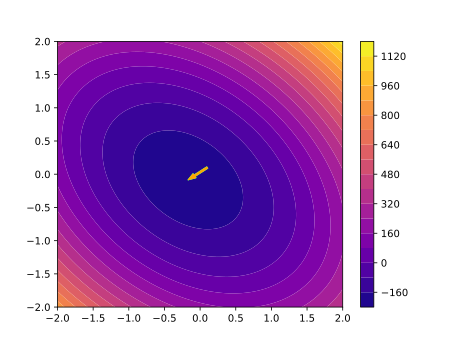
\includegraphics[width=9cm, height=7cm]{img/f3.png}
	      \end{center}

\end{enumerate}

По данным таблиц видно, что первые 2 метода в общем случае не могут найти минимум овражной функции (вторая) и используют во много раз больше итераций для произвольных функций, чем третий метод.
И еще что-нибудь на основе траекторий.

\subsection{Скорость сходимости в зависимости от числа обусловленности и размерности пространства}

\begin{itemize}
	\item Метод градиентного спуска
	      \kngraph{grad}

	\item Метод наискорейшего спуска
	      \kngraph{fast}

	\item Метод сопряженных градиентов
	      \kngraph{conjugate}
\end{itemize}

\section{Выводы}

\section{Графический интерфейс}

\section{Код}

\subsubsection{Вектор}
\mcode{../../include/lab2/vector.h}
\mcode{../../source/lab2/vector.cpp}
\newpage

\subsubsection{Общий класс матриц}
\mcode{../../include/lab2/vector.h}
\mcode{../../source/lab2/vector.cpp}
\newpage

\end{document}

